\documentclass[,jou,floatsintext]{apa6}
\usepackage{lmodern}
\usepackage{amssymb,amsmath}
\usepackage{ifxetex,ifluatex}
\usepackage{fixltx2e} % provides \textsubscript
\ifnum 0\ifxetex 1\fi\ifluatex 1\fi=0 % if pdftex
  \usepackage[T1]{fontenc}
  \usepackage[utf8]{inputenc}
\else % if luatex or xelatex
  \ifxetex
    \usepackage{mathspec}
  \else
    \usepackage{fontspec}
  \fi
  \defaultfontfeatures{Ligatures=TeX,Scale=MatchLowercase}
\fi
% use upquote if available, for straight quotes in verbatim environments
\IfFileExists{upquote.sty}{\usepackage{upquote}}{}
% use microtype if available
\IfFileExists{microtype.sty}{%
\usepackage{microtype}
\UseMicrotypeSet[protrusion]{basicmath} % disable protrusion for tt fonts
}{}
\usepackage{hyperref}
\hypersetup{unicode=true,
            pdftitle={Simulation-Based Power-Analysis for Factorial ANOVA Designs},
            pdfauthor={Daniël Lakens~\& Aaron R. Caldwell},
            pdfkeywords={power analysis, ANOVA, hypothesis test, sample size justification, repeated measures},
            pdfborder={0 0 0},
            breaklinks=true}
\urlstyle{same}  % don't use monospace font for urls
\usepackage{graphicx,grffile}
\makeatletter
\def\maxwidth{\ifdim\Gin@nat@width>\linewidth\linewidth\else\Gin@nat@width\fi}
\def\maxheight{\ifdim\Gin@nat@height>\textheight\textheight\else\Gin@nat@height\fi}
\makeatother
% Scale images if necessary, so that they will not overflow the page
% margins by default, and it is still possible to overwrite the defaults
% using explicit options in \includegraphics[width, height, ...]{}
\setkeys{Gin}{width=\maxwidth,height=\maxheight,keepaspectratio}
\IfFileExists{parskip.sty}{%
\usepackage{parskip}
}{% else
\setlength{\parindent}{0pt}
\setlength{\parskip}{6pt plus 2pt minus 1pt}
}
\setlength{\emergencystretch}{3em}  % prevent overfull lines
\providecommand{\tightlist}{%
  \setlength{\itemsep}{0pt}\setlength{\parskip}{0pt}}
\setcounter{secnumdepth}{0}
% Redefines (sub)paragraphs to behave more like sections
\ifx\paragraph\undefined\else
\let\oldparagraph\paragraph
\renewcommand{\paragraph}[1]{\oldparagraph{#1}\mbox{}}
\fi
\ifx\subparagraph\undefined\else
\let\oldsubparagraph\subparagraph
\renewcommand{\subparagraph}[1]{\oldsubparagraph{#1}\mbox{}}
\fi

%%% Use protect on footnotes to avoid problems with footnotes in titles
\let\rmarkdownfootnote\footnote%
\def\footnote{\protect\rmarkdownfootnote}


  \title{Simulation-Based Power-Analysis for Factorial ANOVA Designs}
    \author{Daniël Lakens\textsuperscript{1}~\& Aaron R. Caldwell\textsuperscript{2}}
    \date{}
  
\shorttitle{ANOVA Power}
\affiliation{
\vspace{0.5cm}
\textsuperscript{1} Human-Technology Interaction Group, Eindhoven University of Technology, The Netherlands\\\textsuperscript{2} Department of Health, Human Performance and Recreation, University of Arkansas, USA}
\keywords{power analysis, ANOVA, hypothesis test, sample size justification, repeated measures\newline\indent Word count: 4654 words.}
\usepackage{csquotes}
\usepackage{upgreek}
\captionsetup{font=singlespacing,justification=justified}

\usepackage{longtable}
\usepackage{lscape}
\usepackage{multirow}
\usepackage{tabularx}
\usepackage[flushleft]{threeparttable}
\usepackage{threeparttablex}

\newenvironment{lltable}{\begin{landscape}\begin{center}\begin{ThreePartTable}}{\end{ThreePartTable}\end{center}\end{landscape}}

\makeatletter
\newcommand\LastLTentrywidth{1em}
\newlength\longtablewidth
\setlength{\longtablewidth}{1in}
\newcommand{\getlongtablewidth}{\begingroup \ifcsname LT@\roman{LT@tables}\endcsname \global\longtablewidth=0pt \renewcommand{\LT@entry}[2]{\global\advance\longtablewidth by ##2\relax\gdef\LastLTentrywidth{##2}}\@nameuse{LT@\roman{LT@tables}} \fi \endgroup}

\authornote{

Correspondence concerning this article should be addressed to Daniël Lakens, ATLAS 9.402, 5600 MB, Eindhoven, The Netherlands. E-mail: \href{mailto:D.Lakens@tue.nl}{\nolinkurl{D.Lakens@tue.nl}}}

\abstract{
Researchers often rely on analysis of variance (ANOVA) when they report results of experiments. To ensure a study is adequately powered to yield informative results when performing an ANOVA, researcher can perform an a-priori power analysis. However, power analysis for factorial ANOVA designs is often a challenge. Current software solutions do not enable power analyses for complex designs with several within-subject factors. Moreover, power analyses often need partial eta-squared or Cohen's f as input, but these effect sizes are not intuitive and do not generalize to different experimental designs. We have created the R package ANOVApower and an online Shiny app to enable researchers without extensive programming experience to perform simulation-based power analysis for ANOVA designs of up to three within- or between-subject factors, with an unlimited number of levels. Predicted effects are entered by specifying means, standard deviations, and correlations (for within-subject factors). The simulation provides the statistical power for all ANOVA main effects, interactions, and individual comparisons, and allow researchers to correct for multiple comparisons. The simulation plots \emph{p}-value distributions for all tests, and power plots across a range of sample sizes. This tutorial will demonstrate how to perform power analysis for ANOVA designs, and highlights important factors that determine the statistical power of factorial ANOVA designs.


}

\begin{document}
\maketitle

When a researcher aims to test hypotheses with an analysis of variance (ANOVA), the sample size of the study should be justified based on the statistical power of the test.
The statistical power of a test is the probability of rejecting the null-hypothesis, given a specified effect size, alpha level, and sample size.
When power is low there is a high probability of concluding there is no effect when the alternative hypothesis is true.
Several excellent resources exist that explain power analyses, including books (Aberson, 2019; Cohen, 1988), general reviews (Maxwell, Kelley, \& Rausch, 2008), and practical primers (Brysbaert, 2019; Perugini, Gallucci, \& Costantini, 2018).
Whereas power analyses for individual comparisons are relatively easy to perform, power analyses for factorial ANOVA designs are a bigger challenge.
Available software solutions do not provide easy options to specify more complex designs (e.g., a 2x2x2 design, where the first factor is manipulated between participants, and the last two factors are manipulated within participants).
The predicted effects often need to be specified as Cohen's f or partial eta squared (\(\eta_p^2\)), which are not the most intuitive way to specify a hypothesized pattern of results, and these effect sizes do not generalize to different experimental designs.
Simulations based on a specified pattern of means and a covariance matrix (based on the expected standard deviation and correlation between within participant factors) provide a more flexible approach to power analyses.
However, such simulations typically require extensive programming knowledge.

In this manuscript we introduce ANOVApower, an R package and Shiny app that can be used to perform power analyses for factorial ANOVA designs based on simulations.
ANOVApower can be used to calculate the statistical power based on a predicted pattern of means, standard deviations, and correlations (for within-subject factors).
By simulating data for factorial designs with specific parameters researchers can gain a better understanding of the factors that determine the statistical power of an ANOVA, and learn how to design well-powered experiments.
After a short introduction to statistical power, focussing on the \emph{F}-test, we will illustrate through simulations how the power of factorial ANOVA designs depend on the pattern of means across conditions, the number of factors and levels, the sample size, and whether you need to control the alpha level for multiple comparisons.

\hypertarget{calculating-power-in-anova-designs}{%
\section{Calculating Power in ANOVA Designs}\label{calculating-power-in-anova-designs}}

Imagine you plan to perform a study in which participants interact with an artificial voice assistant who sounds either cheerful or sad.
You measure how much 80 participants in each condition enjoy to interact with the voice assistant on a line marking scale (coded continuously from -5 to 5) and observe a mean of 0 in the sad condition, and a means of 1 in the cheerful condition, with an estimated standard deviation of 2.
After submitting your manuscript for publication, reviewers ask you to add a study with a neutral control condition to examine whether cheerful voices increase, or sad voices decrease enjoyment (or both).
Depending on what the mean enjoyment in the neutral condition is, what sample size would you need to collect for a high powered test of the expected pattern of means?
A collaborator suggests to switch from a between-subject design to a within-subject design to collect data more efficiently.
What impact will switching from a between-subject to a within-subject design have on the required sample size?
The effect size in the first study could be considered \enquote{medium} based on the benchmarks by Cohen (1988), but does it make sense to plan for a \enquote{medium} effect size in either the between-subject or within-subject ANOVA design?
And if you justify the sample size based on the power for the main effect for the ANOVA, will the study also have sufficient statistical power for the independent comparisons between conditions (or vice versa)?

Let's consider the initial study described above, where enjoyment is measured when 80 participants per condition interact with a cheerful or sad voice assistant.
We can test the difference between two means with a \emph{t}-test or a one-way ANOVA, and the two tests are mathematically equivalent.
Figure \ref{fig:d-plot} and Figure \ref{fig:eta-plot} visualize the distribution of the effect sizes Cohen's d (for the \emph{t}-test) and \(\eta_p^2\) (for the \emph{F}-test) that should be observed when there is no effect (grey curves) and when the observed difference between means equals the true effect (black curves).
In both figures the light grey areas under the null-distribution mark the observed results that would lead to a Type 1 error (observing a statistically significant result if the null-hypothesis is true) and the dark grey areas under the curve marks the observed effect sizes that would lead to a Type 2 error (observing a non-significant result when there is true effect).

\begin{figure}
\centering
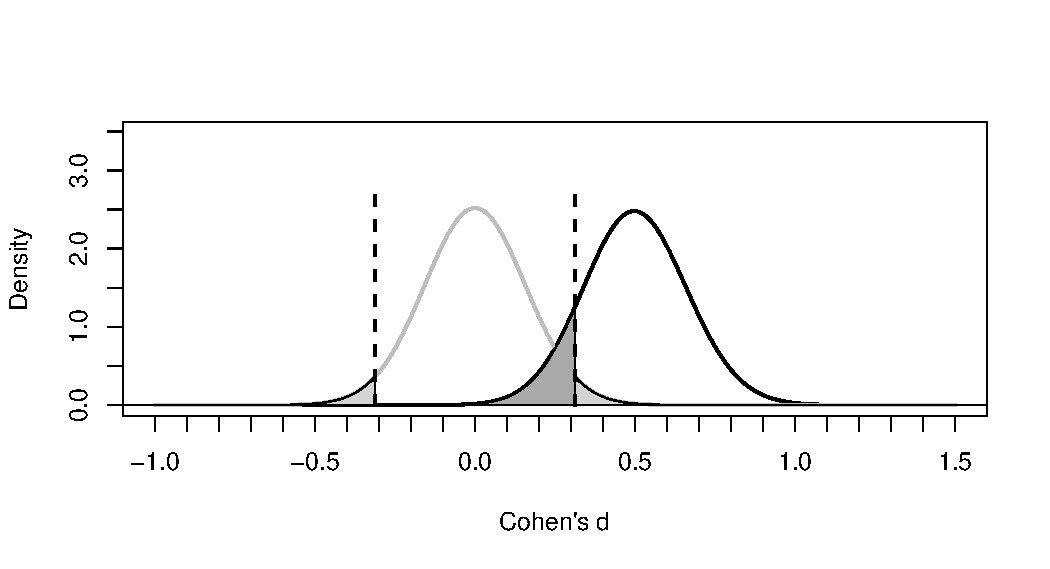
\includegraphics{0.1_Simulation_Based_Power_Analysis_For_Factorial_ANOVA_Designs_files/figure-latex/d-plot-1.pdf}
\caption{\label{fig:d-plot}Distribution of Cohen's d under the null-hypothesis (grey curve) and alternative hypothesis assuming d = 0.5 (black curve).}
\end{figure}

\begin{figure}
\centering
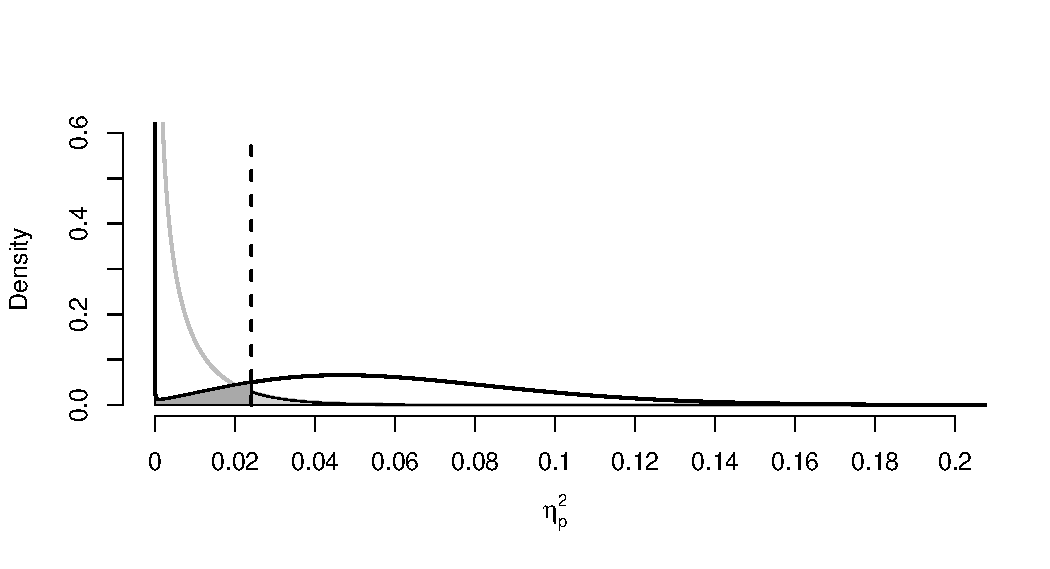
\includegraphics{0.1_Simulation_Based_Power_Analysis_For_Factorial_ANOVA_Designs_files/figure-latex/eta-plot-1.pdf}
\caption{\label{fig:eta-plot}Distribution of eta-squared under the null-hypothesis (grey curve) and alternative hypothesis assuming partial eta-squared = 0.0588 (black curve).}
\end{figure}

When the observed data is more extreme than a critical value, the test result is statistically significant.
Critical values are often expressed as \emph{t}-values or \emph{F}-values, but for a given sample size they can also be expressed as critical \emph{effect sizes}.
Given the sample size of 80 participants per group, observed effects are statistically significant when they are larger than d = 0.31 in a \emph{t}-test, or \(\eta_p^2\) = 0.02 for the \emph{F}-test.
The goal of an a-priori power analysis is to choose a sample size for which the probability of observing a statistically significant effect reaches a desired probability.
To calculate power, one has to specify the alternative hypothesis (the black curves in Figure \ref{fig:d-plot} and \ref{fig:eta-plot}).
If we assume that under the alternative hypothesis the true effect size is d = 0.5 or \(\eta_p^2\) = 0.0588, and data is collected from 80 participants in each condition, in the long run 88.16\% of the observed data will yield statistically significant results.

The \emph{t}-test examines the difference between means \((m_1 - m_2)\), and the \emph{F}-test computes the ratio of the between group variance and the within group variance.
For two groups, the variance of the difference between two means is \((m_1 - m_2)^2\), and therefore \(F = t^2\).
Cohen's d is calculated by dividing the difference between means by the standard deviation, or
\begin{equation}
d = \frac{m_1-m_2}{\sigma}.
\end{equation}
If we have two groups with means of 0 and 1, and the standard deviation is 2, Cohen's d is (1-0)/2, or 0.5.
The generalization of Cohen's d to more than two groups is Cohen's f, which is the standard deviation of the population means divided by the population standard deviation (Cohen, 1988), or:
\begin{equation}
f = \frac{\sigma _{ m }}{\sigma}
\end{equation}
where for equal sample sizes,
\begin{equation}
\sigma _{ m } = \sqrt { \frac { \sum_ { i = 1 } ^ { k } ( m _ { i } - m ) ^ { 2 } } { k } }.
\end{equation}
For two groups Cohen's f is half as large as Cohen's d, or \(f = \frac{1}{2}d\).
Because Cohen's f is the effect size used in power analyses for ANOVA designs it is worth illustrating how Cohen's f is calculated.
If we again take two means of 1 and 2, and a standard deviation of 2, the grand mean is 1.5.
We subtract each condition mean from the grand mean, square it, calculate the sum of squares, divide it by two, and take the square root.
\(\sigma_m = \sqrt{\frac{(0-0.5)^2+(1-0.5)^2}{2}} = \sqrt{\frac{0.25+0.25}{2}} = 0.5\).
Dividing this value by the standard deviation yields \(f = \frac{0.5}{2} = 0.25.\)

G*Power (Faul, Erdfelder, Lang, \& Buchner, 2007) allows researchers to enter the effect size for the power analysis for ANOVA designs as either Cohen's f or partial eta-squared (\(\eta_p^2\)).
Partial eta-squared can be converted into Cohen's f:
\begin{equation}
f = \sqrt{\frac{\eta_p^2}{1-\eta_p^2}} \label{eq:eta-to-f}
\end{equation}
and Cohen's f can be converted into partial eta-squared:
\begin{equation}
\eta_p^2 = \sqrt{\frac{f^2}{f^2+1}} \label{eq:f-to-eta}
\end{equation}
In the example above, \(\eta_p^2 = 0.25^2/(0.25^2+1) = 0.0588\).

Power calculations rely on the noncentrality parameter (lambda, (\(\lambda\)).)
In a between-participants one-way ANOVA lambda is calculated as:
\begin{equation}
\lambda = f^2 \times N \label{eq:lambda}
\end{equation}
where f is Cohen's f and N is the total sample size.
Based on \(\lambda\) (which specifies the shape of the expected distribution under the specified alternative hypothesis, e.g., the black curve in Figure \ref{fig:eta-plot}) and the critical test statistic (which specifies the part of the distribution that is more extreme than the test statistic needed for a statistically significant test result) we can calculate how much of the distribution under the alternative hypothesis will be statistically significant in the long run (i.e., the area under the black curve in Figure \ref{fig:eta-plot} to the right of the critical effect size).

\hypertarget{simulating-statistical-power-for-different-factorial-designs}{%
\section{Simulating Statistical Power for Different Factorial Designs}\label{simulating-statistical-power-for-different-factorial-designs}}

The code underlying the ANOVApower R package and the Shiny app generates data for each condition in the design and performs an ANOVA and \emph{t}-tests for all comparisons between conditions.
The percentage of significant results (i.e., the power) is calculated based on the desired alpha level, and average effect size estimates are computed for all tests.
Users need to specify the design of the study by providing the number of levels for each factor and indicating whether the factor is measured between or within participants.
Our initial study above is a \enquote{2b} or two level between-participant design.
For ease of interpretation the factors and levels can be named (for our example, factor = \enquote{Condition} with levels = \enquote{cheerful} and \enquote{sad}).
The number of observations per condition should be specified (i.e, 80 participants in each between-participant condition).
The means for each condition should be entered (0 and 1), as well as the standard deviation (2).
For within-participant designs the correlation between variables should be specified.
A document detailing how to reproduce all simulations in this manuscript using ANOVApower of the Shiny app is available in the appendix.
For a visual confirmation of the input, a figure is created that displays the means and standard deviation (see Figure \ref{fig:mean-plot2}).

\begin{figure}
\centering
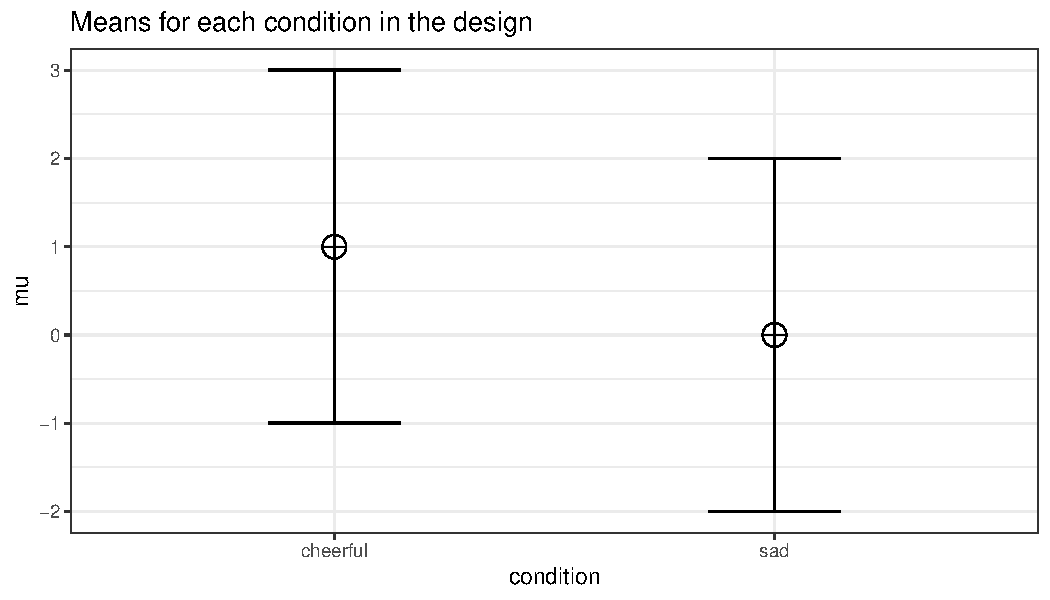
\includegraphics{0.1_Simulation_Based_Power_Analysis_For_Factorial_ANOVA_Designs_files/figure-latex/mean-plot2-1.pdf}
\caption{\label{fig:mean-plot2}Vizualization for the means and standard deviations for the two conditions. Error bars represent one standard deviation.}
\end{figure}

There are two ways to calculate the statistical power of an ANOVA through simulations.
The first is to repeatedly simulate datasets and compute the percentage of statistically significant results.
The second is to simulate a dataset that has \emph{exactly} the desired properties, perform an ANOVA, and use the ANOVA results to compute the statistical power.
The first approach is a bit more flexible, but the second approach is much faster.
ANOVApower let's users choose either of these simulation approaches.
Because the true pattern of the data is unknown in an a-priori power analysis, there is often uncertainty about the values that need to be entered in a power analysis.
It makes sense to examine power across a range of assumptions, from more optimistic scenarios, to more conservative estimates.
It is recommended to power not for the pattern of means you expect, but the smallest effect size that you consider worthwhile to detect (for examples, see Lakens, Scheel, and Isager (2018)).
The results of a simulation study will vary each time the simulation is performed (but can be made reproducible by specifying a \enquote{seed} number).
To perform the simulations, you specify the number of simulations, the alpha level for the tests, and any adjustments for multiple comparisons that are required.
The more simulations that are performed, the more stable the results, but the longer the simulation will take.

If 100.000 simulations are performed for our two group between subjects design with means of 1 and 0, a standard deviation of 2, and 80 participants in each group, with a seed set to 2019 (these settings will be used for all simulation results reported in this manuscript), the statistical power (based on the percentage of \emph{p} \textless{} \(\alpha\) results) is 88.19\% and the average \(\eta_p^2\) is 0.06.
The simulation also provides the results for the individual comparisons based on \emph{t}-tests.
Since there are only two groups in this example, the statistical power for the individual comparison is identical to the ANOVA, but the expected effect size, Cohen's d, is -0.50.

Now that the basic idea behind the simulation is clear, we can use simulations to explore how changes to the experimental design influences power, and answer some of the questions our hypothetical researcher is confronted with when designing a follow-up study.
We will first examine what happens if we add a third, neutral, condition to the design.
Let's assume the mean enjoyment rating for the neutral voice condition falls either perfectly between the cheerful and sad conditions, or is equal to the cheerful condition.
The design now has 3 between-participant conditions, and we can explore what happens if we would collect 80 participants in each condition.

If we assume the mean falls exactly between between the cheerful and sad conditions the simulations show the statistical power for our design is reduced to 81.14\%, and the effect size (partial eta-squared) is 0.05.
If we assume the mean the mean is equal to the cheerful condition, the power increases to 91.03\%.
Compared to the two group design (where the power was 88.19\%), three things have changed.
First, the numerator degrees of freedom has increased because an additional group is added to the design, which makes the non-central \emph{F}-distribution more similar to the central \emph{F}-distribution, which reduces the statistical power.
Second, the total sample size is 50\% larger after adding 80 participants in the third condition, which increases the statistical power of the ANOVA.
Third, the effect size, Cohen's f, has decreased from 0.25 to either 0.20 or \texttt{r\ power\_oneway\_between(design\_result\_2)\$Cohen\_f}, which reduces the statistical power.
The exact effect of these three changes on the statistical power is difficult to predict from one ANOVA design to the next.
The most important conclusion based on these simulations is that changing an experimental design can have several opposing effects on the power of a study, depending of the pattern of means.
One cannot assume the effect size remains unchanged when the design changes, and it might make more sense to think about expected effects in terms of the pattern of means across conditions.

\hypertarget{power-for-within-subject-designs}{%
\section{Power for Within-Subject Designs}\label{power-for-within-subject-designs}}

What happens if we would perform the second study as a within-participants design?
Instead of collecting three groups of participants, we only collect one group, and let this group evaluate the cheerful, neutral, and sad voice assistants.
A rough but useful approximation of the sample size needed in a within-subject design (\(N_W\)), relative to the sample needed in between-design (\(N_B\)), is (from Maxwell \& Delaney, 2004, p.~562, formula 47):
\begin{equation}
N_{W}=\frac{N_{B}(1-\rho)}{a} \label{eq:within-n}
\end{equation}
Here \(a\) is the number of within-participant levels, \(\rho\) is the correlation between the measurements.
Even if the correlation is 0, the required sample size for a within design is reduced because each participants contributes multiple measurements.
A positive correlation reduces the standard deviation of the difference scores and increases the statistical power.
Because the standardized effect size is the mean difference divided by the standard deviation of the difference scores, the correlation has an effect on the standardized mean difference in a within-subject design, referred to as Cohen's \(d_z\) (because it is the effect size of the difference score between \emph{x} and \emph{y}, \emph{z}). The relation is:

\begin{equation}
\sigma_{z}=\sigma\sqrt{2(1-\rho)}
\end{equation}
Cohen's \(d_z\) is used in power analyses for dependent \emph{t}-tests, but there is no equivalent Cohen's \(f_z\) for a within-participant ANOVA, and Cohen's f is identical for within and between designs.
Instead, the value for lambda (\(\lambda\)) is adjusted based on the correlation.
For a one-way within-participant design lambda is identical to Equation \eqref{eq:lambda}, multiplied by \emph{u}, a correction for within-subject designs, calculated as:
\begin{equation}
u = \frac{k}{1-\rho}
\end{equation}
where \(k\) is the number of levels of the within-participant factor, and \(\rho\) is the correlation between dependent variables.
Equations \eqref{eq:eta-to-f} and \eqref{eq:f-to-eta} no longer hold when measurements are correlated.
The default settings in G*Power expects an f or \(\eta_p^2\) that does \emph{not} incorporate the correlation, while the correlation \emph{is} incorporated in the output of software packages such as SPSS.
One can enter the \(\eta_p^2\) from SPSS output in G*Power after checking the \enquote{as in SPSS} checkbox in the options window, but forgetting this is a common mistake in power analyses for within designs in G*Power.
For a one-way within-subject design, Cohen's f can be converted into the Cohen's f SPSS uses through:
\begin{equation}
f^2_{SPSS} = f^2 \times \frac{k}{k-1} \times \frac{n}{n-1} \times \frac{1}{1-\rho}
\end{equation}
and subsequently tranformed to \(\eta_p^2\) through Equation \eqref{eq:f-to-eta}.

Revisting our between-participant design, power was 81.14\% when the enjoyment scores were uncorrelated.
If we want to examine the power for a within design we need to enter a reasonable value for the correlation between dependent variables.
Ideally this value is determined based on previous studies, and it often makes sense to explore a range of possible correlations in an a-priori power analysis.
Let's assume our best estimate of the correlation between enjoyment ratings in a within-subject design is \emph{r} = 0.5.
The power for a repeated-measures ANOVA based on these values, where ratings for the three conditions are collected from 80 participants, is 98.32\%.
Because of the positive correlation between dependent variables, the effect size \(\eta_p^2\) is much larger for the within-subject design (\(\eta_p^2\) = 0.12) than for the 3 group between participants design (\(\eta_p^2\) = 0.05).
Note that the ANOVApower package allow researchers to enter a correlation matrix that specifies the expected correlations between each individual pair of measurements, instead of assuming the correlations between all dependent variables are identical.

\hypertarget{power-for-interactions}{%
\section{Power for Interactions}\label{power-for-interactions}}

The effect size for interactions in ANOVA designs depends on the pattern of means.
Let's assume the researcher plans to perform a follow-up experiment where in addition to making the voice sound cheerful or sad, a second factor is introduced by making the voice sound more robotic compared to the default human-like voice.
Different patterns of results could be expected.
Either the same effect is observed for robotic voices, or no effect is observed for robotic voices, or the opposite effect is observed for robotic voices (we enjoy a sad robotic voice more than a cheerful one, a \enquote{Marvin-the-Depressed-Robot Effect}).
In the first case, we will only observe a main effect of voice, but in the other two scenarios there is an interaction effect between human-likeness of the voice and the emotional tone of the voice.
We can simulate a cross-over interaction for a 2x2 between-participant design with 80 participants in each group to examine the statistical power (see Figure \ref{fig:mean-plot} for the expected pattern of means).

\begin{figure}
\centering
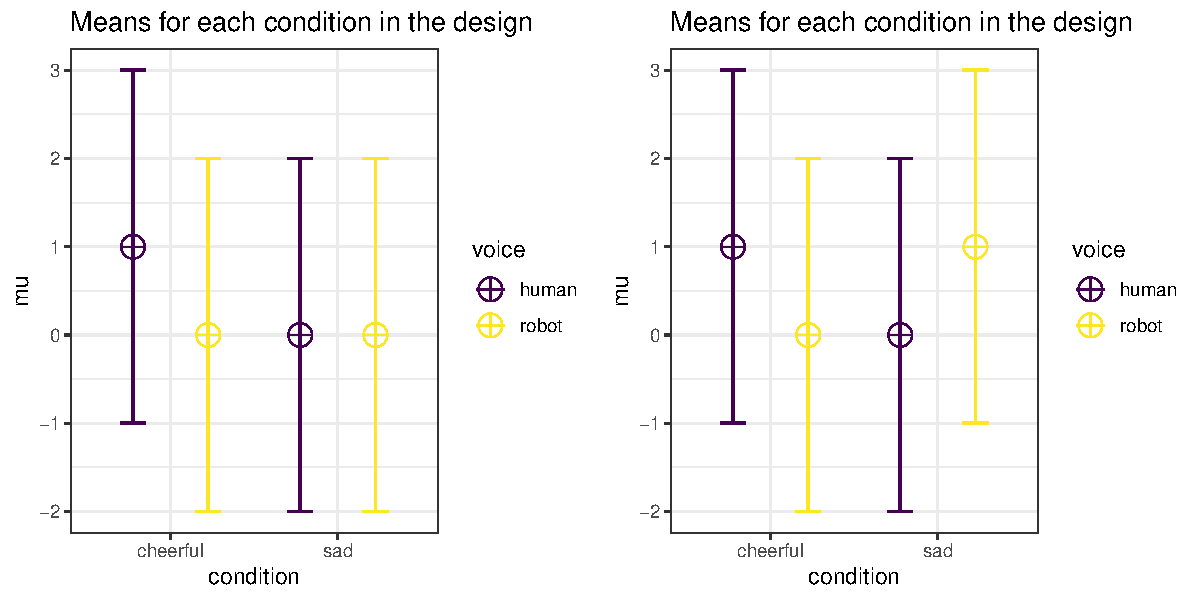
\includegraphics{0.1_Simulation_Based_Power_Analysis_For_Factorial_ANOVA_Designs_files/figure-latex/mean-plot-1.pdf}
\caption{\label{fig:mean-plot}Vizualization for the expected means and standard deviations for a crossover interaction. Error bars represent one standard deviation.}
\end{figure}

Mathematically the interaction effect is computed as the cell mean minus the sum of the grand mean, the marginal mean in each row minus the grand mean, and the marginal mean in each column minus grand mean (see Maxwell, Delaney, and Kelley (2017)). For example, for the cheerful human-like voice condition this is 1 (the value in the cell) - (0.5 {[}the grand mean{]} + 0.5 {[}the cell mean minus the marginal mean in row 1{]} + 0.5 {[}the cell mean minus the marginal mean in column 2{]}).
Thus, 1 - (0.5 + 0.5 + 0.5) = -0.5.
Completing this for all four cells gives the values -0.5, 0.5, 0.5, -0.5.
Cohen's f is then \(f = \frac { \sqrt { \frac { -0.5^2 + 0.5^2 + 0.5 + -0.5^2 } { 4 } }}{ 2 } = 0.25\).
Simulations show we have 99.38\% power when we collect 80 participants per condition.
Power is high, because we collected 80 participants in each condition.
Compared to the two-group comparison with 80 participants per group a cross-over (also called \enquote{disordinal}) interaction with two levels per factor has the same power as the initial two-group design if we halve the sample size per condition (i.e., n = 40 in each cell).
Power with 40 participants per condition is 88.31\%.
Main effects in an ANOVA are based on the means for one factor averaged over the other factors (e.g., the main effect of a human-like versus robot-like voice, irrespective of whether it is cheerful or sad).
The interaction effect can be contrast coded as 1, -1, -1, 1, and thus tests the scores of 80 participants against 80 other participants, just as for the \emph{t}-test or the main effects.
The key insight here is that not the sample size per condition, but the total sample size over all other factors determines the power for the main effects and the interaction (cf.~Westfall, 2015).

We can also examine the statistical power for a pattern of results that indicated that there was no difference in interacting with a cheerful of sad conversational agent with a robot voice.
In this case, we expect an \enquote{ordinal} interaction (the means for the human-like voice are never lower than the means for the robot-like voice, and thus there is no cross-over effect).
The expected pattern of means is 1, 0, 0, 0, with only a single mean that differs from the others.
As has been pointed out (Giner-Sorolla, 2018; Simonsohn, 2014) these designs require larger samples sizes to have the same power to detect the interaction, compared to the two-group comparison.
The reason for this is that the effect size is only half as large, with Cohen's f = 0.125 (compared to 0.25 in the cross-over interaction).

By steadily increasing the sample size in the simulation, we can examine the required sample size to get the same power as for the cross-over interaction with 40 participants per cell (88.31\% power). A total sample size of 635 is required, almost four times as large as the total sample size for the two-group comparison (160). To make it easier to find the sample size per group that is required to calculate the expected power the plot\_power function in ANOVApower can be used to plot the power for a specific design across a range of sample sizes (see Figure \ref{fig:p-plot}).

\begin{figure}
\centering
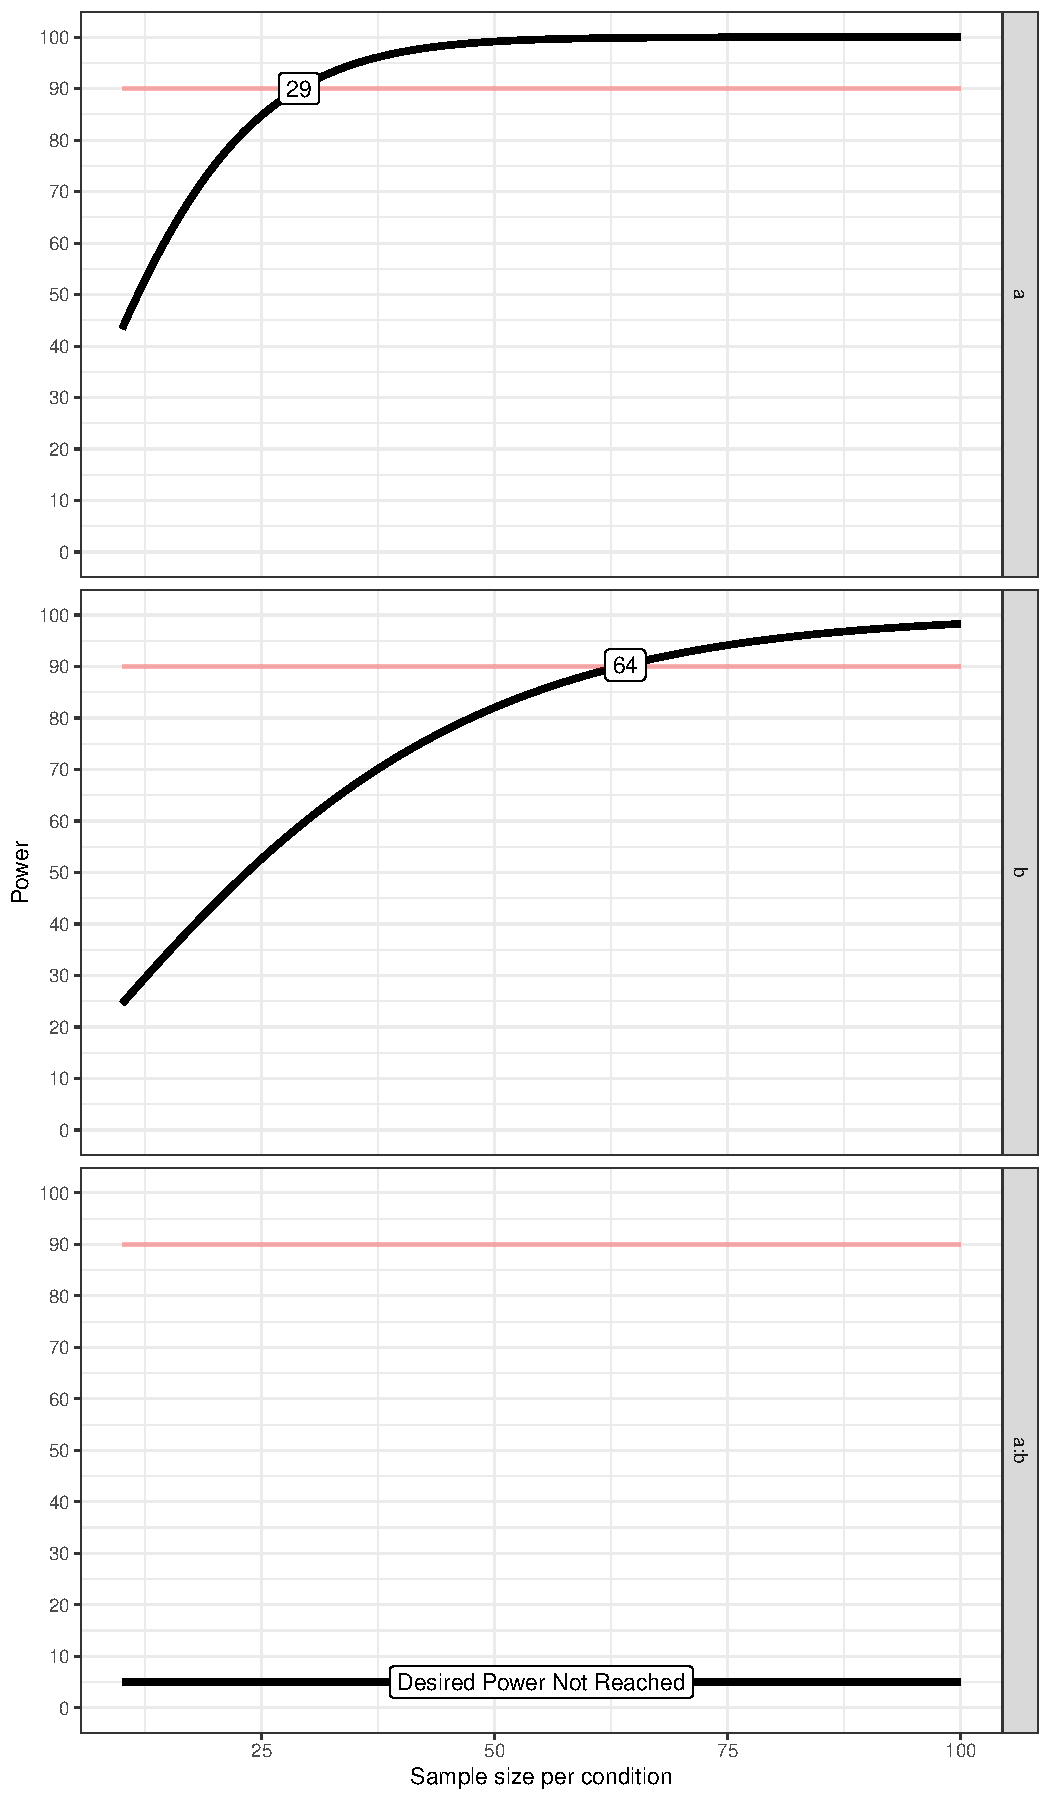
\includegraphics{0.1_Simulation_Based_Power_Analysis_For_Factorial_ANOVA_Designs_files/figure-latex/power-plot-1.pdf}
\caption{\label{fig:power-plot}Power curves across a range of sample sizes per group from n = 10 to n = 200 for the expected main effects and ordinal interaction.}
\end{figure}

Where a two group comparison has a Cohen's f of 0.25 when the means are 1 and 0, a 2x2 ordinal interaction has a Cohen's f of 0.25 when the pattern of means is 2, 0, 0, 0, and a 2x2x2 interaction where only one cell differs from the other means has a Cohen's f of 0.25 when the pattern of means is 4, 0, 0, 0, 0, 0, 0, 0 across the eight cells.
The take-home message is that a \enquote{medium} effect size translates into a much more extreme pattern of means in an ordinal interaction than in a disordinal (crossover) interaction, or in a 2x2x2 interaction compared to a 2x2 interaction (see also Perugini et al. (2018)).
It might therefore be more intuitive to perform a power analysis based on the expected pattern of means, and compute Cohen's f based on this pattern, than to specify an effect size for the power analysis directly.

\hypertarget{power-for-individual-comparisons}{%
\section{Power for Individual Comparisons}\label{power-for-individual-comparisons}}

Although an initial goal when performing an ANOVA might be to test the \emph{omnibus null hypothesis}, which answers the question whether there are \emph{any} differences between group means, we often want to know which conditions differ from each other. Thus, an ANOVA is often followed up by individual comparisons (whether \emph{planned} or \emph{post-hoc}).
One feature of ANOVApower is that it provides the statistical power for all individual comparisons that can be performed.
The power and effect size estimates are based on simple \emph{t}-tests.
Taking into account the variance estimates from other groups (which the \emph{t}-tests do not do) can have power benefits (Maxwell et al., 2017), but these depend on whether the homogeneity assumption is met, which is often not warranted in psychological research, and violations of the homogeneity assumption impact Type 1 error rates (Delacre, Lakens, Mora, \& Leys, 2018).\\
Furthermore, performing individual \emph{t}-tests as follow-up tests allow researchers to specify directional predictions which increase the power of individual comparisons.

Power analysis for individual comparisons is relatively straightforward and can easily be done in all power analysis software, but providing power for all individual comparisons alongside the ANOVA hopefully nudges researchers to take into account the power for follow-up tests.
Sometimes the interaction in the ANOVA will have more power than the individual comparisons (i.e., in the case of a cross-over interaction) and sometimes the power for the interaction will be lower than the power for independent comparisons.
It is always important to check if you have adequate power for all tests you plan to perform, which includes main effects, interactions, and individual comparisons performed as follow-up tests.

\hypertarget{type-1-error-control-in-exploratory-anovas}{%
\section{Type 1 Error Control in Exploratory ANOVA's}\label{type-1-error-control-in-exploratory-anovas}}

In a 2x2x2 design, an ANOVA will give the test results for three main effects, three two-way interactions, and one three-way interaction.
Because seven statistical tests are performed, the probability of making at least one Type 1 error in a single exploratory 2x2x2 ANOVA is \(1-(0.95)^7\) = 30\%.
It is therefore important to control error rates when performing multiple comparisons (Cramer et al., 2016).

It is possible to control the overall Type I error rate by specifying an adjustment for multiple comparisons in the simulation.
By adjusting for multiple comparisons we ensure that we do not conclude there is an effect in \emph{any} of the individual tests more often than the desired Type I error rate.
Several techniques to control error rates exist, of which the best known is the Bonferroni adjustment.
The Holm procedure is slightly more powerful than the Bonferroni adjustment, without requiring additional assumptions (for other approaches, see Bretz, Hothorn, \& Westfall, 2011).
Because the adjustment for multiple comparisons lowers the alpha level, it also lowers the statistical power.
When designing a study where you will perform multiple comparisons, it is important to take into account the corrected alpha level when determining the required sample size, both for the ANOVA tests, as for the individual comparisons.

If we revisit the 2x2 between-condition ANOVA where a cross-over interaction was predicted and 40 participants per condition were collected, and apply a Holm correction for multiple comparisons, we see power for the interaction is reduced from 88.31\% without applying a correction, to 77.28\% after correcting for multiple comparisons.
There are three tests for a 2x2 design (two main effects, one interaction), but 6 individual comparisons between the four conditions, and thus the correction for multiple comparisons has a stronger effect on the individual comparisons.
For example, the power for the \emph{t}-test comparing two between-participant conditions falls from 60.17\% without correcting for multiple comparisons, to 35.86\% when adjusting the alpha level for the 6 possible individual comparisons between the four conditions.

These simulations should reveal the cost (in terms of the statistical power) of exploring across all possible comparisons while controlling error rates.
It is often advisable to preregister specific tests that are of interest to a researcher.
If one is really interested in all possible comparisons, but wants to control the probability of incorrectly acting as if there is an effect, the reduction in power due to the lower alpha level should be counteracted by increasing the sample size to maintain an adequate level of power for both the ANOVA as the individual comparisons.

\hypertarget{p-value-distributions}{%
\section{P-value distributions}\label{p-value-distributions}}

Statistical power is the long run probability of observing a \emph{p}-value smaller than the alpha level.
One intuitive way to illustrate this concept is to plot the distribution of \emph{p}-values for all simulations.
The simulation code automatically stores plots for \emph{p}-value distributions for each test in the simulation.
In Figure \ref{fig:p-plot} we see that for the initial 2 group between-participant design most \emph{p}-values fall below the alpha level (in the figure, the vertical line as 0.05).
For the 1e+05 simulations, 88.19\% fall below the alpha level.
As power is increased the p-value distribution becomes steeper, and when there is an effect size of zero \emph{p}-values are uniformly distributed.

\begin{figure}
\centering
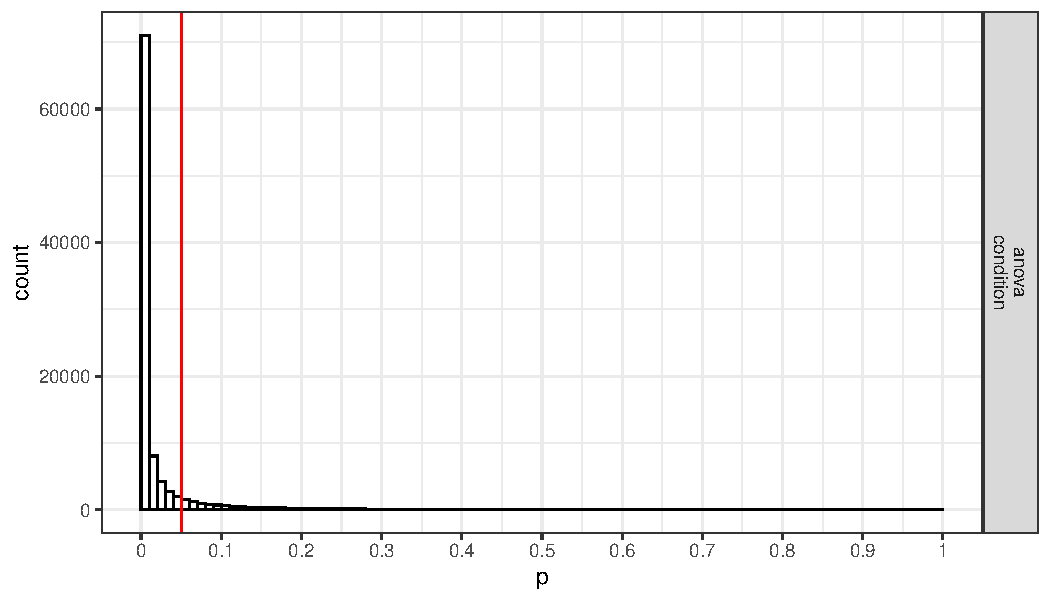
\includegraphics{0.1_Simulation_Based_Power_Analysis_For_Factorial_ANOVA_Designs_files/figure-latex/p-plot-1.pdf}
\caption{\label{fig:p-plot}Distribution of p-values for the initial two-group between subjects design.}
\end{figure}

\hypertarget{conclusion}{%
\section{Conclusion}\label{conclusion}}

It is important to carefully justify the sample size when designing informative studies.
Simulation based approaches can help to provide insights into the factors that determine the statistical power for factorial ANOVA designs.
Exploring the power for designs with specific patterns of means, standard deviations, and correlations between variables can be used to choose a design and sample size that provides the highest statistical power for future studies. The R package (\url{https://github.com/Lakens/ANOVApower}) and Shiny app (\url{http://shiny.ieis.tue.nl/anova_power/}) that accompany this paper enable researchers to perform simulations for factorial experiments of up to three factors and any number of levels, making it easy to perform simulation-based power analysis without extensive programming experience.

\hypertarget{author-contributions}{%
\subsection{Author Contributions}\label{author-contributions}}

D. Lakens and A. R. Caldwell collaboratively developed the ANOVApower R package. D. Lakens wrote the initial draft, and both authors revised the manuscript. A. R. Caldwell created the Shiny app.

\hypertarget{orcid-ids}{%
\subsection{ORCID iD's}\label{orcid-ids}}

Daniël Lakens 
\includegraphics{screenshots/orcid.png} \url{https://orcid.org/0000-0002-0247-239X}
Aaron R. Caldwell 
\includegraphics{screenshots/orcid.png} \url{https://orcid.org/0000-0002-4541-6283}

\hypertarget{acknowledgements}{%
\subsection{Acknowledgements}\label{acknowledgements}}

Many improvements to ANOVApower are based on feedback from Lisa DeBruine and the sim\_design function in her \enquote{faux} R package. The ANOVA\_exact function was inspired by Chris Aberson. We are grateful to Jonathon Love for the development of a jamovi module based on ANOVApower.

\hypertarget{declaration-of-conflicting-interests}{%
\subsection{Declaration of Conflicting Interests}\label{declaration-of-conflicting-interests}}

The author(s) declared that there were no conflicts of interest with respect to the authorship or the publication of this article.

\hypertarget{funding}{%
\subsection{Funding}\label{funding}}

This work was funded by VIDI Grant 452-17-013 from the Netherlands Organisation for Scientific Research.

\hypertarget{open-practices}{%
\subsection{Open Practices}\label{open-practices}}

The code to reproduce the analyses reported in this article has been made publicly available via the Open Science Framework and can be accessed at \url{https://osf.io/pn8mc/}.

\hypertarget{references}{%
\section{References}\label{references}}

\setlength{\parindent}{-0.5in}
\setlength{\leftskip}{0.5in}

\hypertarget{refs}{}
\leavevmode\hypertarget{ref-aberson_applied_2019}{}%
Aberson, C. L. (2019). \emph{Applied Power Analysis for the Behavioral Sciences} (2nd ed.). New York: Routledge.

\leavevmode\hypertarget{ref-bretz_multiple_2011}{}%
Bretz, F., Hothorn, T., \& Westfall, P. H. (2011). \emph{Multiple comparisons using R}. Boca Raton, FL: CRC Press.

\leavevmode\hypertarget{ref-brysbaert_how_2019}{}%
Brysbaert, M. (2019). How many participants do we have to include in properly powered experiments? A tutorial of power analysis with some simple guidelines. \emph{Journal of Cognition}.

\leavevmode\hypertarget{ref-cohen_statistical_1988}{}%
Cohen, J. (1988). \emph{Statistical power analysis for the behavioral sciences} (2nd ed.). Hillsdale, N.J: L. Erlbaum Associates.

\leavevmode\hypertarget{ref-cramer_hidden_2016}{}%
Cramer, A. O. J., van Ravenzwaaij, D., Matzke, D., Steingroever, H., Wetzels, R., Grasman, R. P. P. P., \ldots{} Wagenmakers, E.-J. (2016). Hidden multiplicity in exploratory multiway ANOVA: Prevalence and remedies. \emph{Psychonomic Bulletin \& Review}, \emph{23}(2), 640--647. doi:\href{https://doi.org/10.3758/s13423-015-0913-5}{10.3758/s13423-015-0913-5}

\leavevmode\hypertarget{ref-delacre_why_2018}{}%
Delacre, M., Lakens, D., Mora, Y., \& Leys, C. (2018). Why Psychologists Should Always Report the W-test Instead of the F-Test ANOVA. \emph{PsyArXiv}. doi:\href{https://doi.org/10.17605/OSF.IO/WNEZG}{10.17605/OSF.IO/WNEZG}

\leavevmode\hypertarget{ref-faul_gpower_2007}{}%
Faul, F., Erdfelder, E., Lang, A.-G., \& Buchner, A. (2007). GPower 3: A flexible statistical power analysis program for the social, behavioral, and biomedical sciences. \emph{Behavior Research Methods}, \emph{39}(2), 175--191. doi:\href{https://doi.org/10.3758/BF03193146}{10.3758/BF03193146}

\leavevmode\hypertarget{ref-giner-sorolla_powering_2018}{}%
Giner-Sorolla, R. (2018, January). Powering Your Interaction. \emph{Approaching Significance}. https://approachingblog.wordpress.com/2018/01/24/powering-your-interaction-2/.

\leavevmode\hypertarget{ref-lakens_equivalence_2018}{}%
Lakens, D., Scheel, A. M., \& Isager, P. M. (2018). Equivalence Testing for Psychological Research: A Tutorial. \emph{Advances in Methods and Practices in Psychological Science}, \emph{1}(2), 259--269. doi:\href{https://doi.org/10.1177/2515245918770963}{10.1177/2515245918770963}

\leavevmode\hypertarget{ref-maxwell_designing_2017}{}%
Maxwell, S. E., Delaney, H. D., \& Kelley, K. (2017). \emph{Designing Experiments and Analyzing Data: A Model Comparison Perspective, Third Edition} (3rd ed.). New York, NY: Routledge.

\leavevmode\hypertarget{ref-maxwell_sample_2008}{}%
Maxwell, S. E., Kelley, K., \& Rausch, J. R. (2008). Sample Size Planning for Statistical Power and Accuracy in Parameter Estimation. \emph{Annual Review of Psychology}, \emph{59}(1), 537--563. doi:\href{https://doi.org/10.1146/annurev.psych.59.103006.093735}{10.1146/annurev.psych.59.103006.093735}

\leavevmode\hypertarget{ref-perugini_practical_2018}{}%
Perugini, M., Gallucci, M., \& Costantini, G. (2018). A Practical Primer To Power Analysis for Simple Experimental Designs. \emph{International Review of Social Psychology}, \emph{31}(1), 20. doi:\href{https://doi.org/10.5334/irsp.181}{10.5334/irsp.181}

\leavevmode\hypertarget{ref-simonsohn_no-way_2014}{}%
Simonsohn, U. (2014, March). No-way Interactions. \emph{Data Colada}. http://datacolada.org/17.

\leavevmode\hypertarget{ref-westfall_think_2015}{}%
Westfall, J. (2015, May). Think about total N, not n per cell. \emph{Cookie Scientist}. http://jakewestfall.org/blog/index.php/2015/05/26/think-about-total-n-not-n-per-cell/.


\end{document}
